% ==============================================
% ELEMENTO: DESENVOLVIMENTO
% ==============================================
\section{Desenvolvimento}
\label{sec:desenvolvimento}

% ========== Alínea a) ==========
\subsection{Dimensionamento do andar de saída}
\label{subsec:andar_saida}

A primeira parte deste trabalho consiste em dimensionar o andar de saída do buffer.
O objetivo é escolher os valores de $C_D$ e $g_{m11}$ de forma a cumprir as especificações do
\textit{settling error} (inferior a 0,05\%, ou seja, 0,55~mV) e da queda inicial provocada pela
ligação de $C_{DAC}$ (inferior a 50~mV).

\begin{figure}[H]
    \centering
    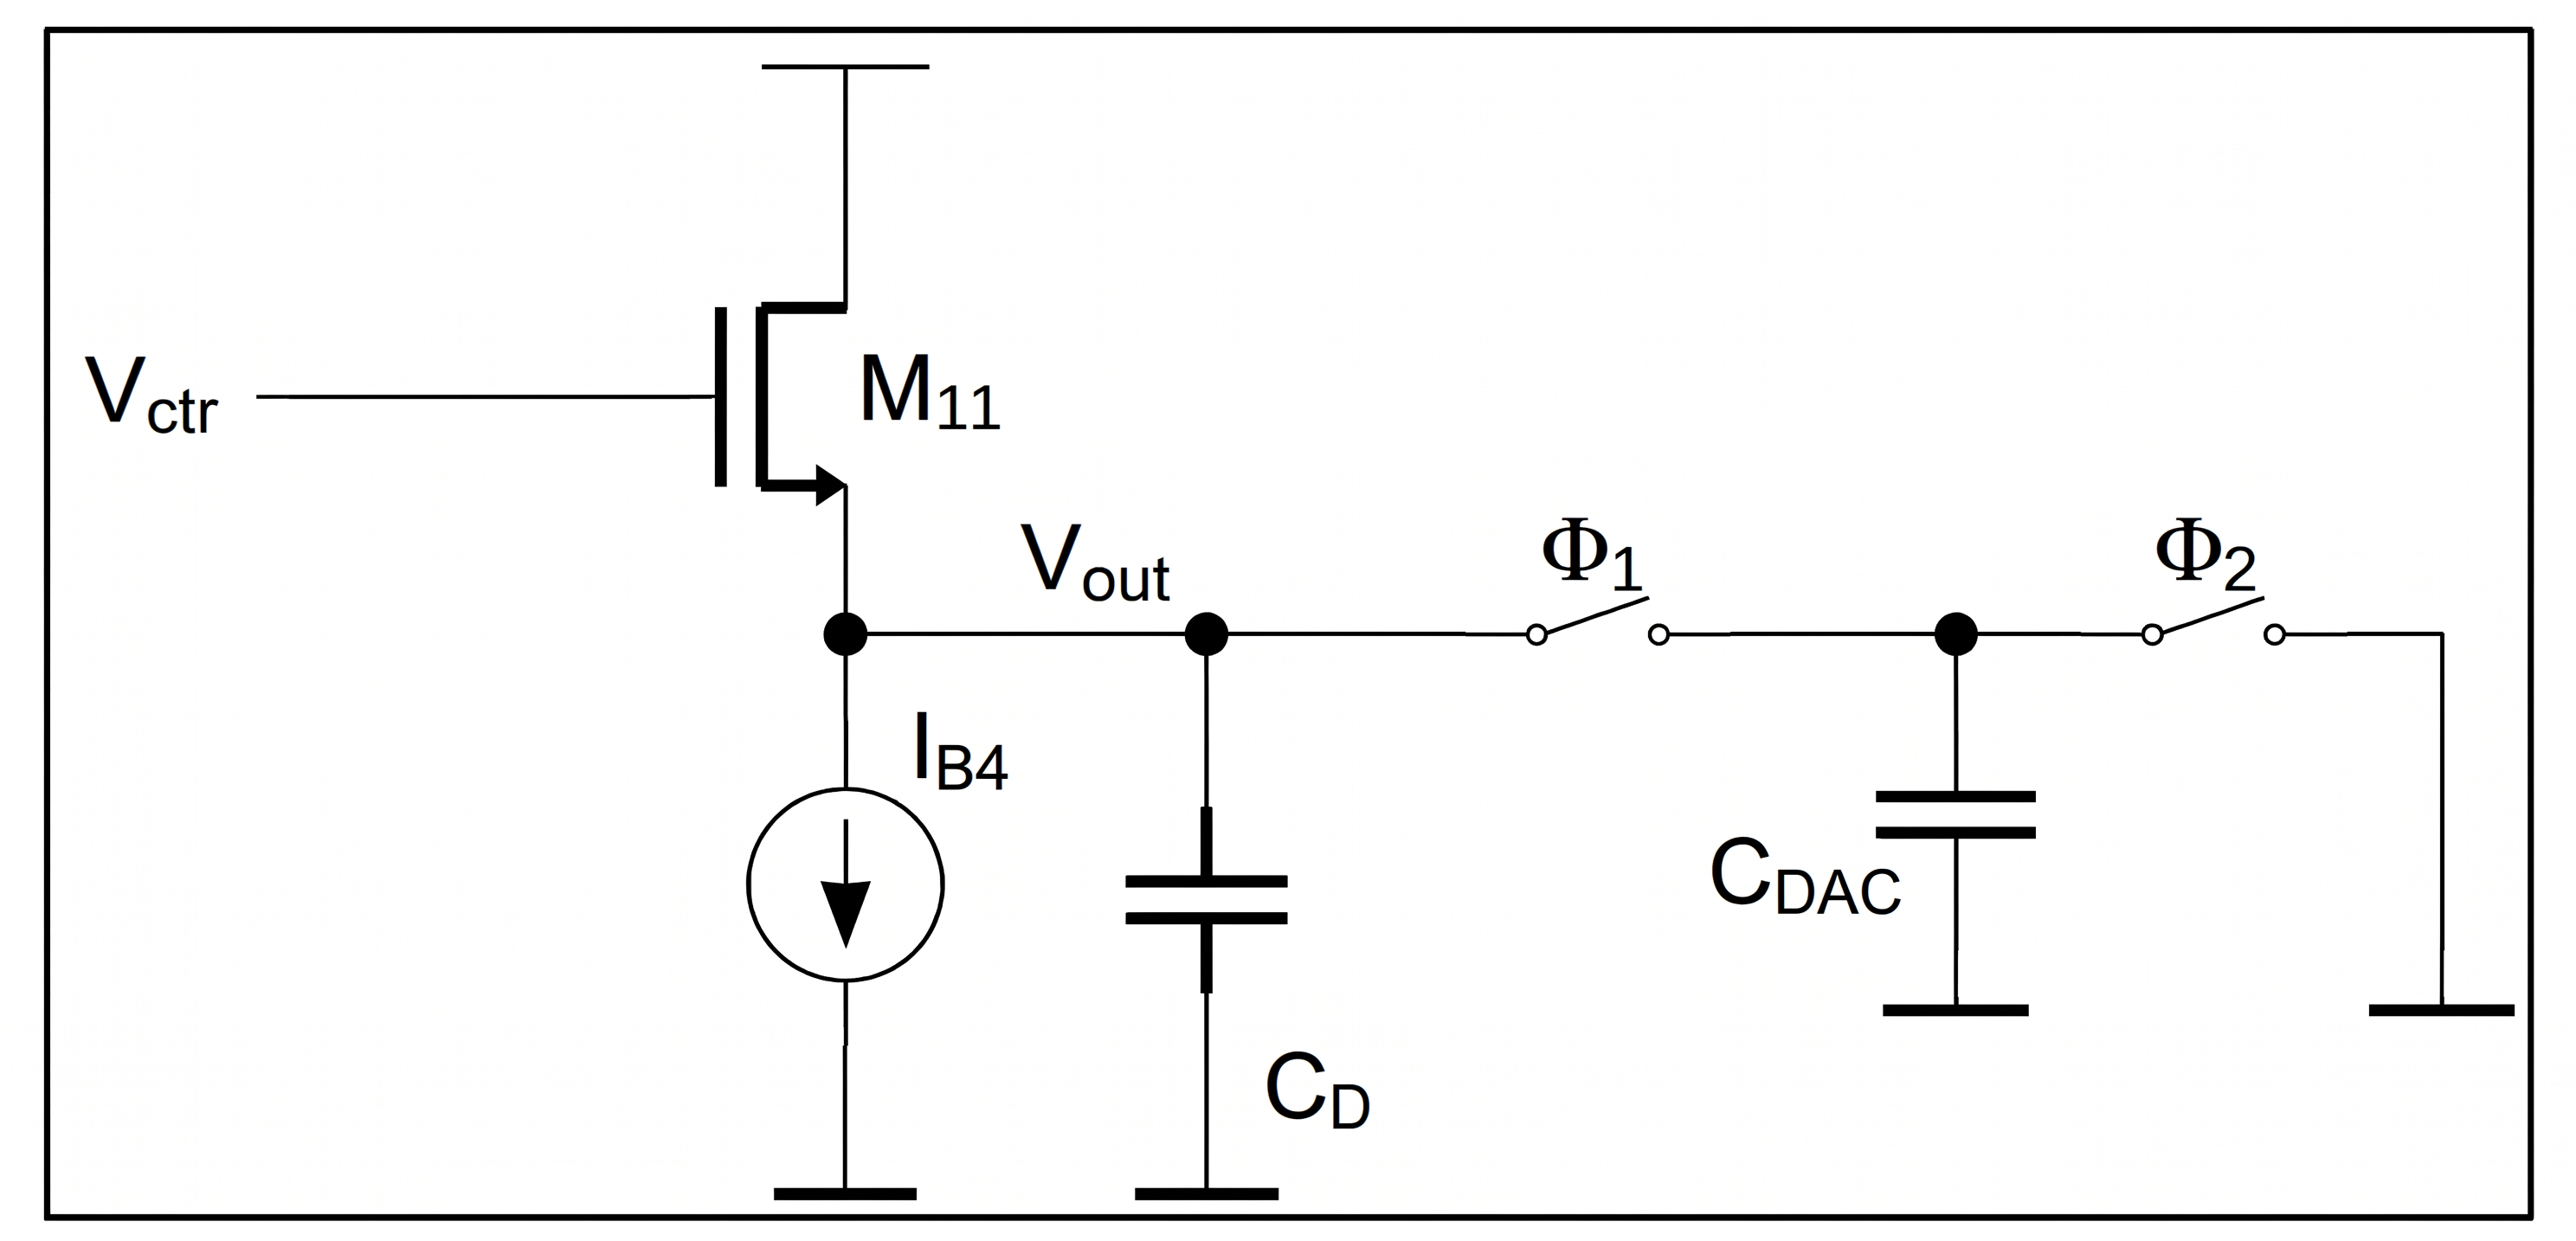
\includegraphics[width=0.8\linewidth]{IMAGENS/primeiro circuito.png}
    \caption{Circuito simplificado do andar de saída.}
    \label{fig:dimensionamento_M11}
\end{figure}

Comecemos então por analisar o circuito simplificado da figura \ref{fig:dimensionamento_M11} em pequenos sinais,
permitindo-nos obter uma expressão para a impedância de saída.

Aplicando a lei dos nós em $v_{out}$, com a gate de $M_{11}$ em ground em AC, temos ($v_{gs11} = -v_{out}$) e designando por $i_{DAC}$ a corrente retirada pelo $C_{DAC}$:
\begin{equation}
    -g_{m11}\,v_{gs11} + g_{ds11}\,v_{out} + sC_D\,v_{out} + i_{DAC} = 0
\end{equation}

pelo que a impedância de saída do seguidor é
\begin{equation}
    Z_{out}(s) = -\frac{v_{out}}{i_{DAC}} = \frac{1}{g_{m11} + g_{ds11} + sC_D}
    \label{eq:zout_seguidor}
\end{equation}

Quando $\Phi_1$ fecha, $C_{DAC}$ (inicialmente descarregado) é ligado a $v_{out}$. Em pequeno sinal,
em torno de $V_{ref}$, a sua tensão inicial é $-V_{ref}$, pelo que a corrente que retira do nó é
\begin{equation}
    i_{DAC}(s) = sC_{DAC}\,v_{out}(s) + C_{DAC}V_{ref}
\end{equation}

onde o termo $C_{DAC}V_{ref}$ corresponde à carga retirada instantaneamente pela partilha de carga.
Substituindo na equação do nó:
\begin{equation}
    v_{out}(s)\left[g_{m11} + g_{ds11} + s\left(C_D + C_{DAC}\right)\right] = -\,C_{DAC}V_{ref}
\end{equation}

Definindo $C = C_D + C_{DAC}$:

\begin{equation}
    v_{out}(s) = -\frac{V_{ref}\,C_{DAC}}{C}\cdot\frac{1}{s + \dfrac{g_{m11}+g_{ds11}}{C}}
\end{equation}

e, aplicando a transformada de Laplace inversa,

\begin{equation}
    v_{out}(t) = -\frac{V_{ref}\,C_{DAC}}{C_D + C_{DAC}}\;e^{-\frac{g_{m11}+g_{ds11}}{C_D + C_{DAC}}\,t}
    \label{eq:vout_t}
\end{equation}

A queda inicial é, portanto, $\Delta V = V_{ref}\,C_{DAC}/(C_D + C_{DAC})$, e a constante de tempo do settling é
$\tau = (C_D + C_{DAC})/(g_{m11}+g_{ds11})$.

Como diz no enunciado do trabalho, temos uma frequência de clock de 250~MHz, pelo que o período de relógio é $T_{clk} = 4$~ns.
A especificação do settling error ($< 0{,}55$~mV) traduz-se em:
\begin{equation}
    \left|v_{out}(T_{clk})\right| = \frac{V_{ref}\,C_{DAC}}{C_D + C_{DAC}}\;e^{-\frac{g_{m11}+g_{ds11}}{C_D + C_{DAC}}\,T_{clk}} < \varepsilon\,V_{ref}
    \label{eq:cond_erro}
\end{equation}

com $\varepsilon = 5\times10^{-4}$ (0,05\%). Isolando a transcondutância:
\begin{equation}
    g_{m11} + g_{ds11} > \frac{C_D + C_{DAC}}{T_{clk}}\,\ln\!\left(\frac{C_{DAC}}{\varepsilon\,\left(C_D + C_{DAC}\right)}\right)
\end{equation}
Considerando, numa primeira aproximação, $g_{ds11} = g_{m11}/10$:
\begin{equation}
    g_{m11} > \frac{C_D + C_{DAC}}{1{,}1\,T_{clk}}\,\ln\!\left(\frac{C_{DAC}}{\varepsilon\,\left(C_D + C_{DAC}\right)}\right)
    \label{eq:gm_min}
\end{equation}

Para escolher $C_D$ e $g_{m11}$, implementou-se em Python a Eq.~\eqref{eq:gm_min}, percorrendo valores de $C_D$ entre 1 e 20~pF.
Para cada valor calculou-se o $g_{m11}$ mínimo que garante um erro de 0,55~mV ao fim de $T_{clk} = 4$~ns, a corrente correspondente
(para $g_m/I_D = 28$) e a queda inicial $\Delta V$.

O valor de $g_m/I_D$ define a relação entre a transcondutância e a corrente de polarização. Como $g_{m11}$ está fixado pelas especificações,
a corrente necessária é $I_{B4} = g_{m11}/(g_m/I_D)$, pelo que um $g_m/I_D$ elevado minimiza a potência dissipada. Em inversão fraca, $g_m/I_D$
tende para o seu valor máximo, $1/(n\,U_T) \approx 30$~V$^{-1}$ (com $n \approx 1{,}3$ e $U_T \approx 26$~mV), que não é atingível na prática.
Escolheu-se $g_m/I_D = 28$~V$^{-1}$, próximo deste limite, de modo a obter a menor corrente possível sem levar o transístor a inversão fraca profunda.


Os resultados estão resumidos na Tabela~\ref{tab:varrimento_cd}.

\begin{table}[H]
    \centering
    \caption{$g_{m11}$ mínimo, corrente e queda inicial em função de $C_D$ ($T_{clk} = 4$~ns, erro $= 0{,}55$~mV).}
    \label{tab:varrimento_cd}
    \begin{tabular}{ccccc}
        \toprule
        $C_D$ [pF] & $g_{m11,min}$ [mS] & $I_D$ [$\mu$A] & $\Delta V$ [mV] & $\Delta V \le 50$~mV \\
        \midrule
        8  & 9,21  & 329 & 64,7 & não \\
        9  & 10,05 & 359 & 57,9 & não \\
        10 & 10,87 & 388 & 52,4 & não \\
        11 & 11,67 & 417 & 47,8 & sim \\
        12 & 12,45 & 445 & 44,0 & sim \\
        13 & 13,21 & 472 & 40,7 & sim \\
        14 & 13,95 & 498 & 37,9 & sim \\
        15 & 14,68 & 524 & 35,5 & sim \\
        16 & 15,39 & 550 & 33,3 & sim \\
        \bottomrule
    \end{tabular}
\end{table}


\begin{figure}[H]
    \centering
    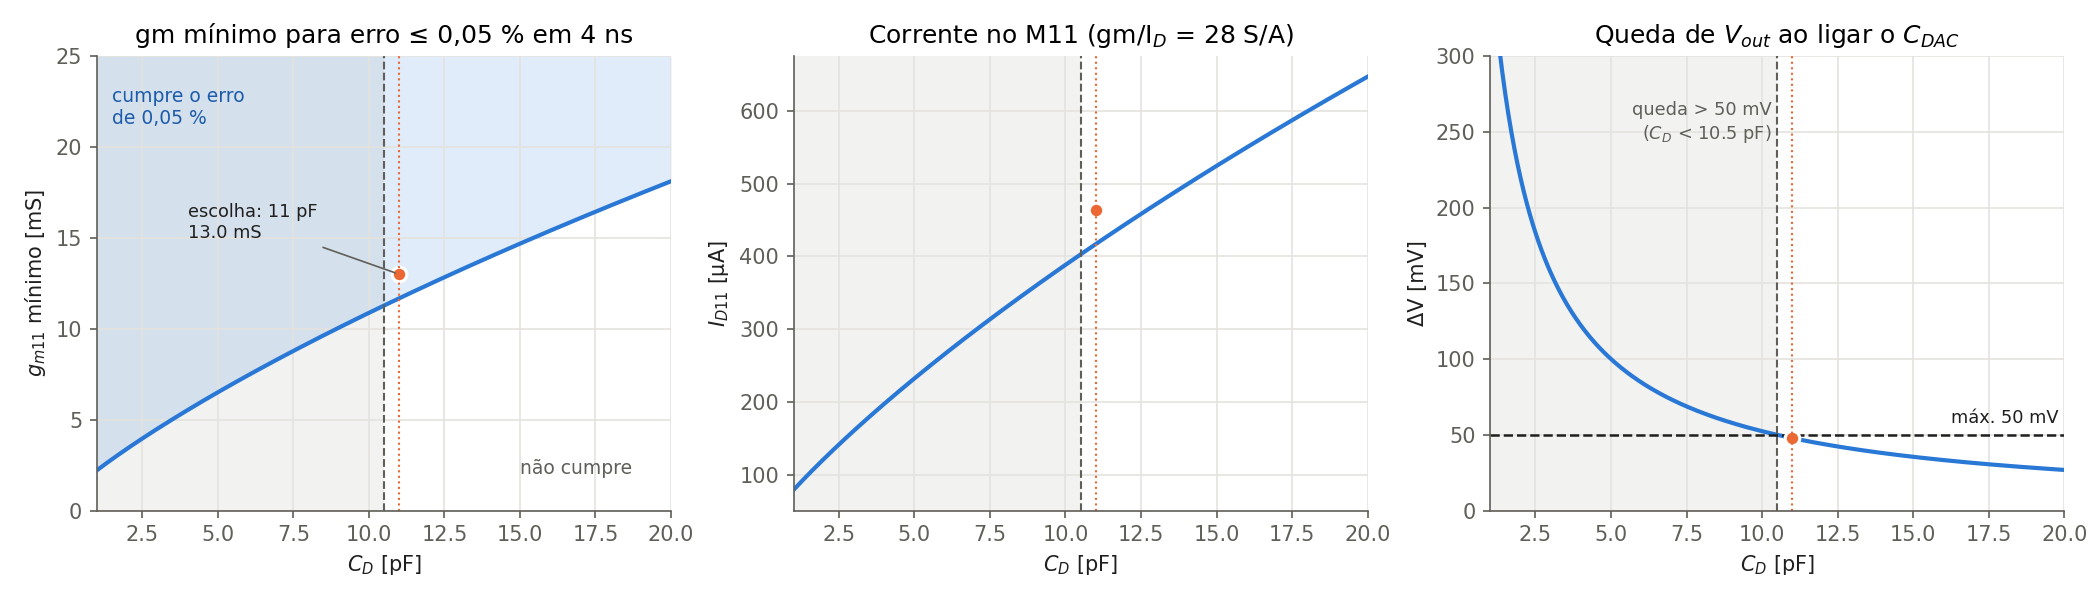
\includegraphics[width=\linewidth]{IMAGENS/fig1_gm_vs_CD.png}
    \caption{Compromisso entre $C_D$, $g_{m11}$, corrente e queda inicial.}
    \label{fig:compromisso_cd_gm}
\end{figure}

A Fig.~\ref{fig:compromisso_cd_gm} evidencia o compromisso entre as duas especificações: a queda inicial impõe $C_D \ge 10{,}5$~pF, enquanto o $g_{m11}$ mínimo, e com ele a corrente, cresce com $C_D$.

\begin{figure}[H]
    \centering
    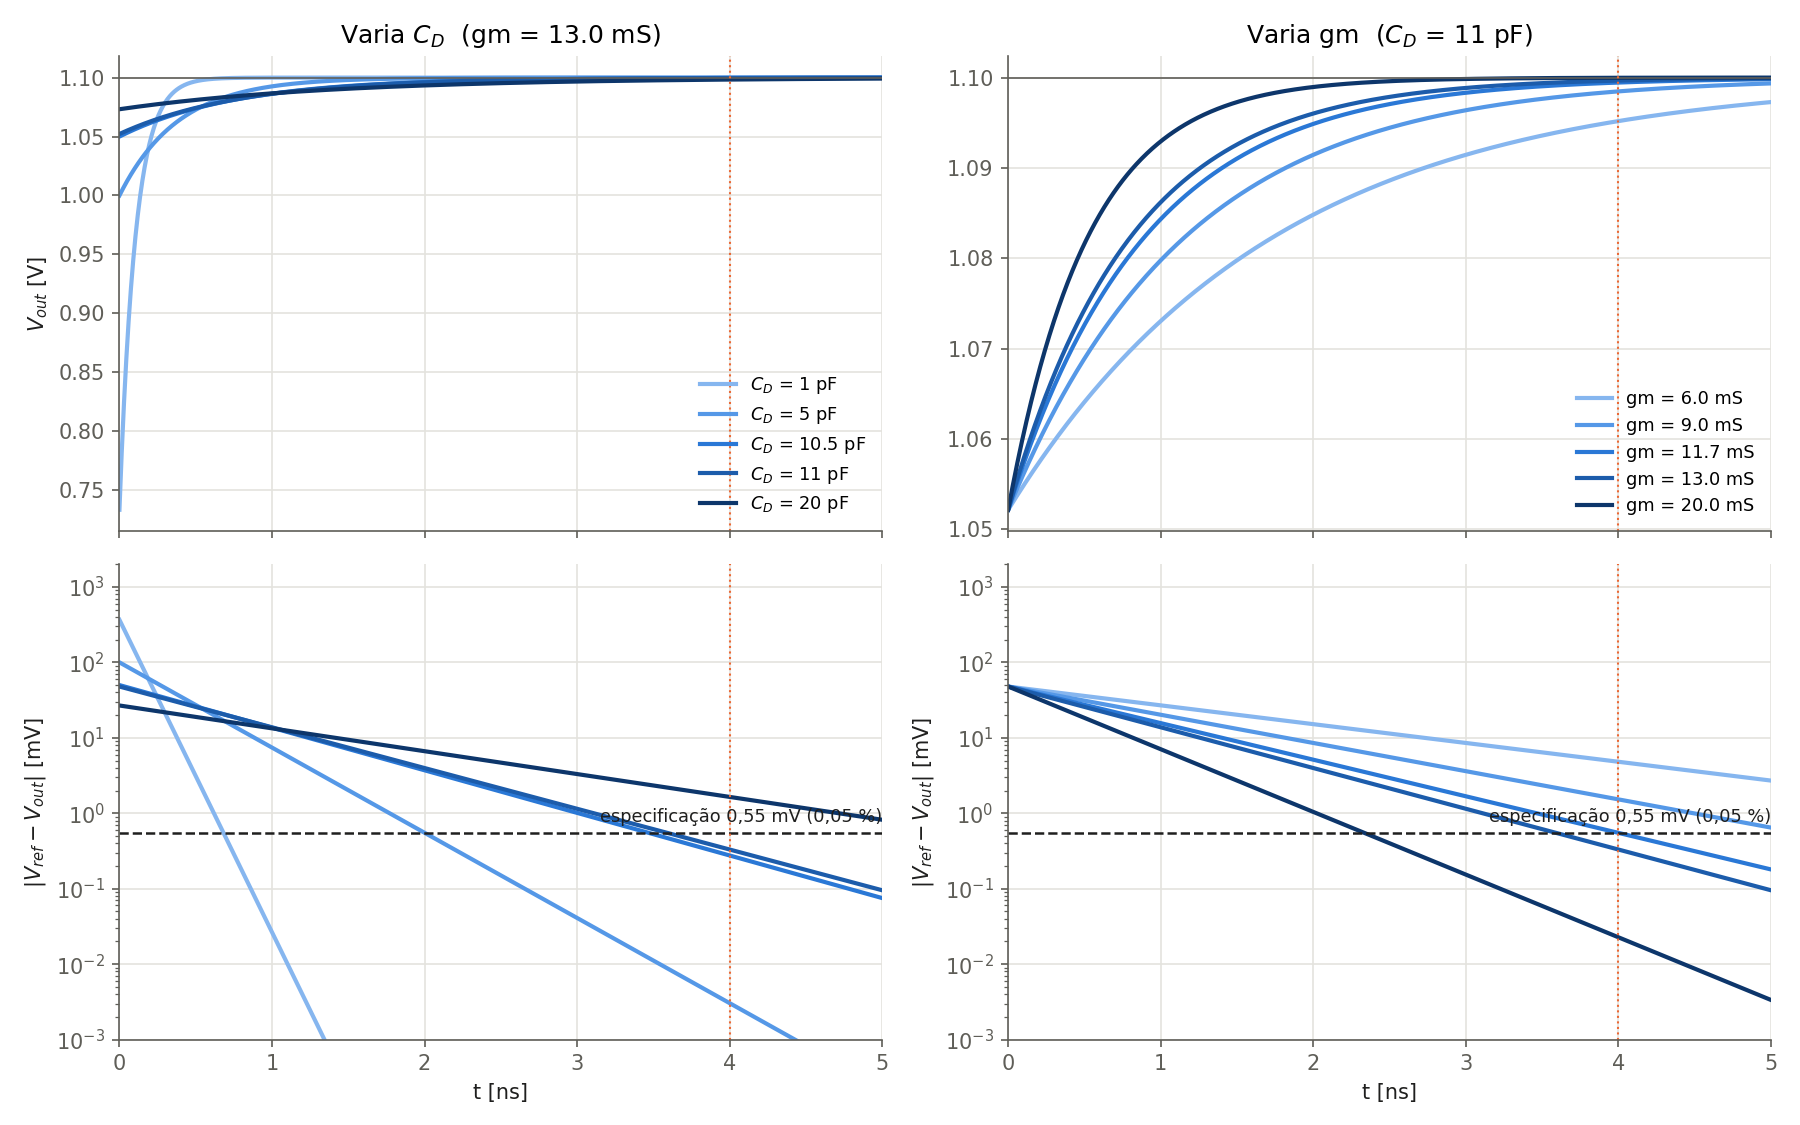
\includegraphics[width=\linewidth]{IMAGENS/fig2_Vout_t.png}
    \caption{Variação de $C_D$ ($g_{m11} = 13$~mS) e variação de $g_{m11}$ ($C_D = 11$~pF): resposta de $V_{out}$ e erro $|V_{ref} - V_{out}|$.}
    \label{fig:transitorio_teorico}
\end{figure}

A Fig.~\ref{fig:transitorio_teorico} mostra a resposta temporal de $v_{out}$ prevista pela Eq.~\eqref{eq:vout_t}: aumentar $C_D$ reduz a queda inicial mas torna o assentamento mais lento, enquanto aumentar $g_{m11}$ acelera o assentamento sem alterar a queda.

\begin{figure}[H]
    \centering
    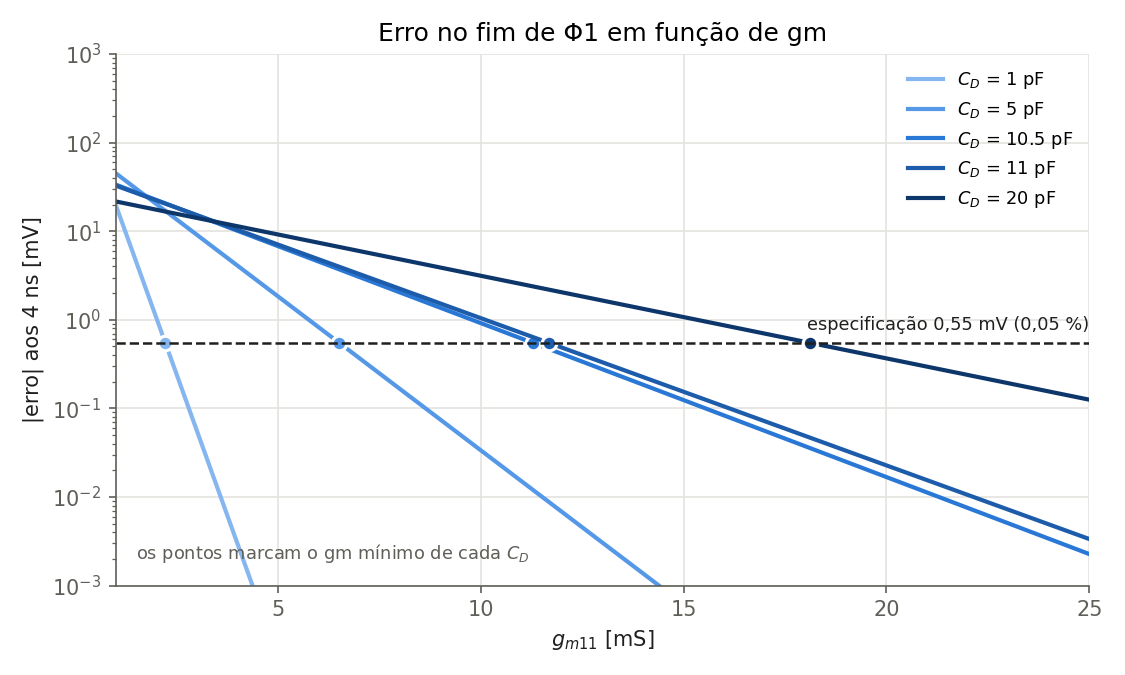
\includegraphics[width=0.8\linewidth]{IMAGENS/fig3_erro_vs_gm.png}
    \caption{Erro aos 4~ns em função de $g_{m11}$, para vários valores de $C_D$. Os pontos marcam o $g_{m11}$ mínimo de cada $C_D$.}
    \label{fig:erro_vs_gm}
\end{figure}

\begin{figure}[H]
    \centering
    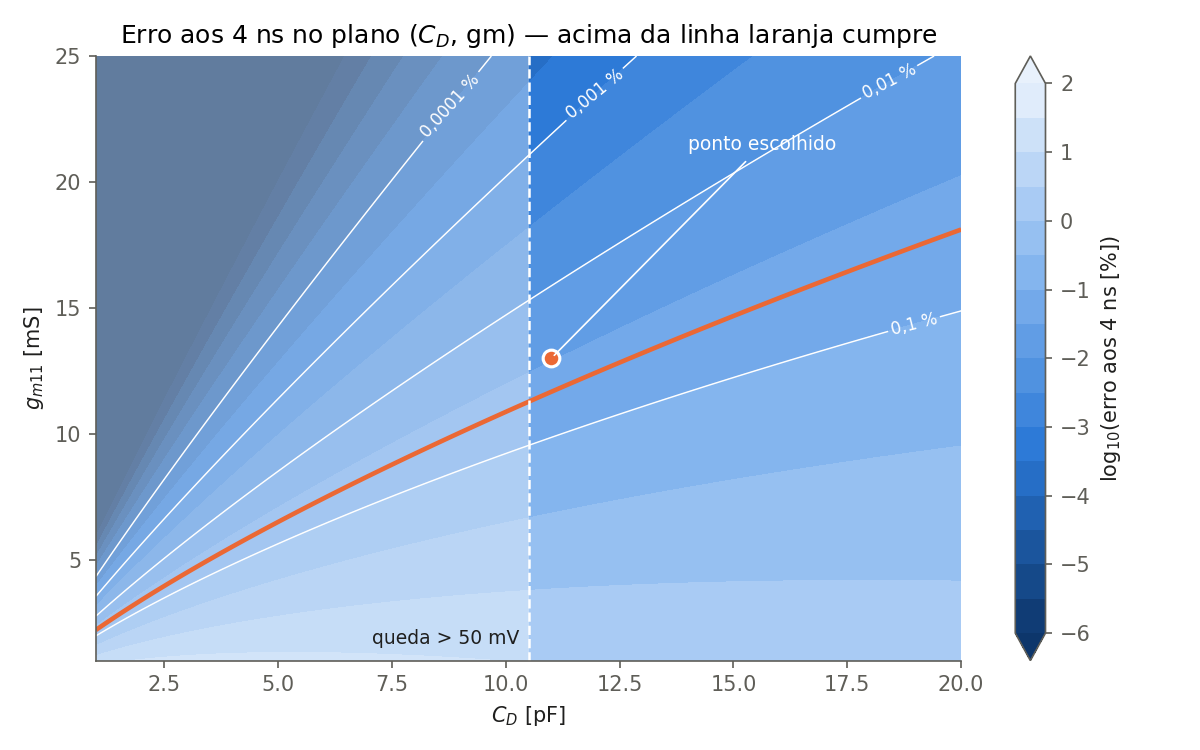
\includegraphics[width=0.8\linewidth]{IMAGENS/fig4_mapa_CD_gm.png}
    \caption{Erro aos 4~ns no plano ($C_D$, $g_{m11}$): acima da linha laranja cumpre a especificação.}
    \label{fig:mapa_erro}
\end{figure}

A Fig.~\ref{fig:erro_vs_gm} mostra o erro aos 4~ns em função de $g_{m11}$, assinalando o valor mínimo para cada $C_D$, e a Fig.~\ref{fig:mapa_erro} resume a região do plano ($C_D$, $g_{m11}$) que cumpre a especificação, com o ponto escolhido.

Verifica-se que $C_D = 11$~pF é o menor valor inteiro que cumpre a especificação da queda inicial, exigindo $g_{m11} \ge 11{,}67$~mS.
Valores superiores de $C_D$ reduzem a queda mas aumentam o $g_{m11}$ e, consequentemente, a corrente necessária.
Escolheu-se assim $C_D = 11$~pF e, para garantir margem no settling error, $g_{m11} = 13$~mS. Com estes valores obtém-se:
\begin{itemize}
    \item queda inicial: $\Delta V = 47{,}8$~mV ($< 50$~mV);
    \item erro ao fim de 4~ns: $0{,}331$~mV ($< 0{,}55$~mV);
    \item $V_{out}(4\text{ ns}) = 1{,}099669$~V;
    \item corrente de polarização: $I_{B4} = g_{m11}/(g_m/I_D) = 13\text{m}/28 \approx 464~\mu$A.
\end{itemize}
Estes valores serviram de ponto de partida para o dimensionamento do $M_{11}$ em simulação.

% ========== Cadence para o M11 ==========
\subsubsection{Validação em simulação}
\label{subsubsec:validacao_m11}

\begin{figure}[H]
    \centering
    
\includegraphics[width=0.6\linewidth]{IMAGENS/m11 cadence circuito.png}
    \caption{Circuito de teste do andar de saída no Cadence.}
    \label{fig:m11_circuito_cadence}
\end{figure}

O dimensionamento anterior foi validado no Cadence com o circuito da Fig.~\ref{fig:m11_circuito_cadence}. O seguidor $M_{11}$ foi implementado com um
transístor \texttt{nch\_25\_dnw} ($L = 280$~nm, $W = 2~\mu$m $\times$ 5 \textit{fingers}), com o \textit{bulk} ligado à source para eliminar o
efeito de corpo, que aumentaria $V_{GS11}$ e o tornaria dependente de $V_{out}$, e polarizado com $I_{B4} = 464~\mu$A. A gate é polarizada por uma fonte DC ideal, que representa
$V_{ctr}$, ajustada de modo a obter $V_{out} \approx 1{,}1$~V. O $C_{DAC}$ é ligado e descarregado por dois interruptores comandados por relógio
não sobrepostos: $\Phi_1$ (ligação a $V_{out}$, de 0,1 a 1,9~ns) e $\Phi_2$ (descarga, de 2 a 4~ns), com período de 4~ns. O settling error é medido no fim
do período, em relação ao valor de repouso de $V_{out}$.

Mantendo $I_{B4}$ e $C_D = 11$~pF, variou-se o tamanho de $M_{11}$ através do multiplicador $M$ (de 50 a 900). A Tabela~\ref{tab:sweep_M} resume alguns dos
pontos obtidos.

\begin{table}[H]
    \centering
    \caption{Erro no fim de $\Phi_1$ e no fim do período em função do multiplicador $M$ de $M_{11}$ ($C_D = 11$~pF).}
    \label{tab:sweep_M}
    \begin{tabular}{ccc}
        \toprule
        $M$ & Erro fim de $\Phi_1$ [mV] & Erro fim do período [mV] \\
        \midrule
        70  & 7,10 & 0,99 \\
        170 & 6,57 & 0,97 \\
        210 & 6,53 & 0,97 \\
        350 & 6,76 & 1,29 \\
        890 & 7,52 & 2,05 \\
        \bottomrule
    \end{tabular}
\end{table}

O erro apresenta um mínimo para $M \approx 210$. Para valores superiores, o $g_{m11}$ quase não aumenta, porque o transístor está próximo da inversão fraca
e o $g_m/I_D$ satura, enquanto as capacidades de gate continuam a crescer e tornam a resposta mais lenta. Escolheu-se, assim, $M = 210$.

Mesmo com este valor, o erro no fim do período ($\approx 0{,}97$~mV) ultrapassa a especificação ($0{,}55$~mV). Isto deve-se às capacidades do próprio
$M_{11}$: com a gate em ground em AC, $C_{gs11}$ e $C_{gb11}$ ficam em paralelo com $C_D$, pelo que a capacidade total no nó de saída é superior à
considerada na análise teórica. Para compensar, com $M = 210$, variou-se $C_D$ entre 7,75 e 8,75~pF (Tabela~\ref{tab:sweep_cd_sim}).

\begin{table}[H]
    \centering
    \caption{Queda inicial e erro no fim do período em função de $C_D$ ($M = 210$).}
    \label{tab:sweep_cd_sim}
    \begin{tabular}{cccc}
        \toprule
        $C_D$ [pF] & Queda [mV] & Erro [$\mu$V] & Cumpre \\
        \midrule
        7,75 & 50,7 & 442 & não (queda) \\
        8,00 & 49,6 & 482 & sim \\
        8,25 & 48,5 & 531 & sim \\
        8,50 & 47,5 & 569 & não (erro) \\
        \bottomrule
    \end{tabular}
\end{table}

Escolheu-se $C_D = 8{,}25$~pF, que apresenta margem nas duas especificações. A partir da queda medida, a capacidade total no nó de saída é $C_{total}
\approx V_{out}C_{DAC}/\Delta V \approx 11{,}3$~pF, ou seja, cerca de 2,5~pF acima de $C_D + C_{DAC}$. Esta diferença corresponde às capacidades de $M_{11}$
ligadas a $V_{out}$, que funcionam como uma capacidade adicional. A capacidade efetiva é, por isso, $C_{D,ef} \approx 10{,}8$~pF, coerente com o mínimo de
10,5~pF obtido na análise teórica.

O ponto de funcionamento final de $M_{11}$ está resumido na Tabela~\ref{tab:op_m11}.

\begin{table}[H]
    \centering
    \caption{Ponto de funcionamento de $M_{11}$ ($M = 210$, $C_D = 8{,}25$~pF).}
    \label{tab:op_m11}
    \begin{tabular}{cc}
        \toprule
        Parâmetro & Valor \\
        \midrule
        $I_D$ & 464~$\mu$A \\
        $V_{GS}$ & 453,6~mV \\
        $g_{m11}$ & 11,22~mS \\
        $g_{ds11}$ & 367~$\mu$S \\
        $g_m/I_D$ & 24,2~V$^{-1}$ \\
        $g_m/g_{ds}$ & 30,6 \\
        $|C_{gs11}|$ & 1,15~pF \\
        $|C_{gd11}|$ & 0,77~pF \\
        $|C_{gg11}|$ & 2,42~pF \\
        Queda inicial & 48,5~mV \\
        Erro no fim do período & 531~$\mu$V (0,048\%) \\
        \bottomrule
    \end{tabular}
\end{table}

Note-se que o $M_{11}$ resultante é um transístor grande ($W_{total} = 2{,}1$~mm), com $C_{gg11} \approx 2{,}4$~pF.
Esta capacidade fica ligada a $V_{ctr}$, ou seja, à saída do amplificador, e vai afetar a estabilidade e a resposta no
tempo do circuito completo. Este dimensionamento é, por isso, um ponto de partida: o tamanho de $M_{11}$ (e, com ele, o valor de $C_D$)
poderá ser revisto após o dimensionamento do amplificador, se necessário.

% ========== Dimensionamento do M1 ==========
\subsubsection{Dimensionamento da réplica $M_1$}
\label{subsubsec:dimensionamento_m1}

O transístor $M_1$ é uma réplica de $M_{11}$: o amplificador força $V_{outR} = V_{ref}$ e, como $M_1$ e $M_{11}$ partilham a tensão de gate
$V_{ctr}$, $V_{out}$ acompanha $V_{outR}$ desde que ambos tenham a mesma tensão $V_{GS}$. Para isso, os dois transístores têm de ser do mesmo
tipo, ter o mesmo comprimento $L$ e operar com a mesma densidade de corrente:
\begin{equation}
    \frac{I_{B3}}{W_1} = \frac{I_{B4}}{W_{11}} \quad\Rightarrow\quad W_1 = \frac{W_{11}}{K}, \qquad I_{B3} = \frac{I_{B4}}{K}
\end{equation}
onde $K$ é um fator de escala. Um $K$ elevado reduz a corrente e a capacidade que a réplica introduz em $V_{ctr}$, mas aumenta o \textit{mismatch}
entre $M_1$ e $M_{11}$ e, consequentemente, o \textit{offset} entre $V_{out}$ e $V_{outR}$.

Optou-se por $K = 1$, que garante o melhor emparelhamento entre os dois seguidores. Assim, $M_1$ é idêntico a $M_{11}$ (\texttt{nch\_25\_dnw}, \textit{bulk} ligado à source,
$L = 280$~nm, $W = 2~\mu$m $\times$ 5 \textit{fingers}, $M = 210$) e polarizado com $I_{B3} = 464~\mu$A.
Em simulação, ambos apresentam $V_{GS} = 453{,}7$~mV, pelo que, no ponto de funcionamento,
\begin{equation}
    V_{ctr} = V_{ref} + V_{GS11} \approx 1{,}1 + 0{,}454 = 1{,}554~\text{V}
\end{equation}
Em contrapartida, esta escolha duplica a corrente consumida pelos seguidores e a capacidade ligada a
$V_{ctr}$ ($C_{gg1} \approx C_{gg11} \approx 2{,}4$~pF), o que é tido em conta no dimensionamento do amplificador.

% ========== Alíneas b), c) e d) ==========
\subsection{Análise do amplificador}
\label{subsec:analise_amp}

\subsubsection{Circuito simplificado e modelo de pequeno sinal}

Após o dimensionamento do andar de saída, analisa-se o amplificador que controla $V_{ctr}$.
Para tornar a análise tratável, consideram-se as seguintes simplificações sobre o circuito da Fig.~\ref{fig:circuito}:
\begin{itemize}
    \item como o par diferencial é simétrico, analisa-se apenas o meio-circuito do lado de $M_{1B}$ (ramo de $V_x$);
    \item a fonte de cauda ($M_{4B}$) é substituída por uma fonte de corrente ideal $I_{B1}$;
    \item as gates das fontes de corrente ($M_{3B}$ e $M_4$) e da cascode ($M_{2B}$) estão ligadas a tensões de
    polarização fixas ($V_{BN}$, $V_{B4}$ e $V_{B3}$), pelo que são ground AC.
\end{itemize}

\begin{figure}[H]
    \centering
    \includegraphics[width=0.8\linewidth]{IMAGENS/circuito_simplificado_sem_Iextra.png}
    \caption{Circuito simplificado do amplificador.}
    \label{fig:amplificador_simplificado}
\end{figure}

O circuito resultante, representado na Fig.~\ref{fig:amplificador_simplificado}, é um amplificador de dois andares.
O primeiro andar é formado por $M_{1B}$ com a carga em cascode $M_{2B}$--$M_{3B}$, e o segundo pelo andar de fonte
comum $M_5$ com a carga ativa $M_4$. O condensador $C_C$ liga $V_{ctr}$ à fonte de $M_{2B}$ (nó de baixa impedância),
o que corresponde a uma compensação indireta. A saída do amplificador ($V_{ctr}$) controla o seguidor réplica $M_1$,
cuja fonte ($V_{outR}$) fecha a malha de realimentação.

Para a análise em pequeno sinal consideram-se as capacidades parasitas de todos os transístores, representadas na
Fig.~\ref{fig:amplificador_parasitas}. Os nós de interesse são $V_1$ ($= V_x$), $V_2$ ($= V_{ctr}$), $V_3$ (fonte
de $M_{2B}$) e $V_{outR}$. A carga de $M_{11}$ e de $M_{1A}$, que não estão representados, é incluída através das
capacidades $C_{gg11}$, no nó $V_{ctr}$, e $C_{gs1A}$ e $C_{gd1A}$, no nó $V_{outR}$.

Além do condensador de compensação $C_C$, o circuito sugerido inclui um condensador $C_P$ no nó $V_{ctr}$. Ao
contrário das restantes, esta não é uma capacidade parasita, mas um elemento de projeto, que é incluído na análise
como parte do nó $V_{ctr}$. O seu valor é discutido no dimensionamento (Secção~\ref{subsec:gmid}).

\begin{figure}[H]
    \centering
    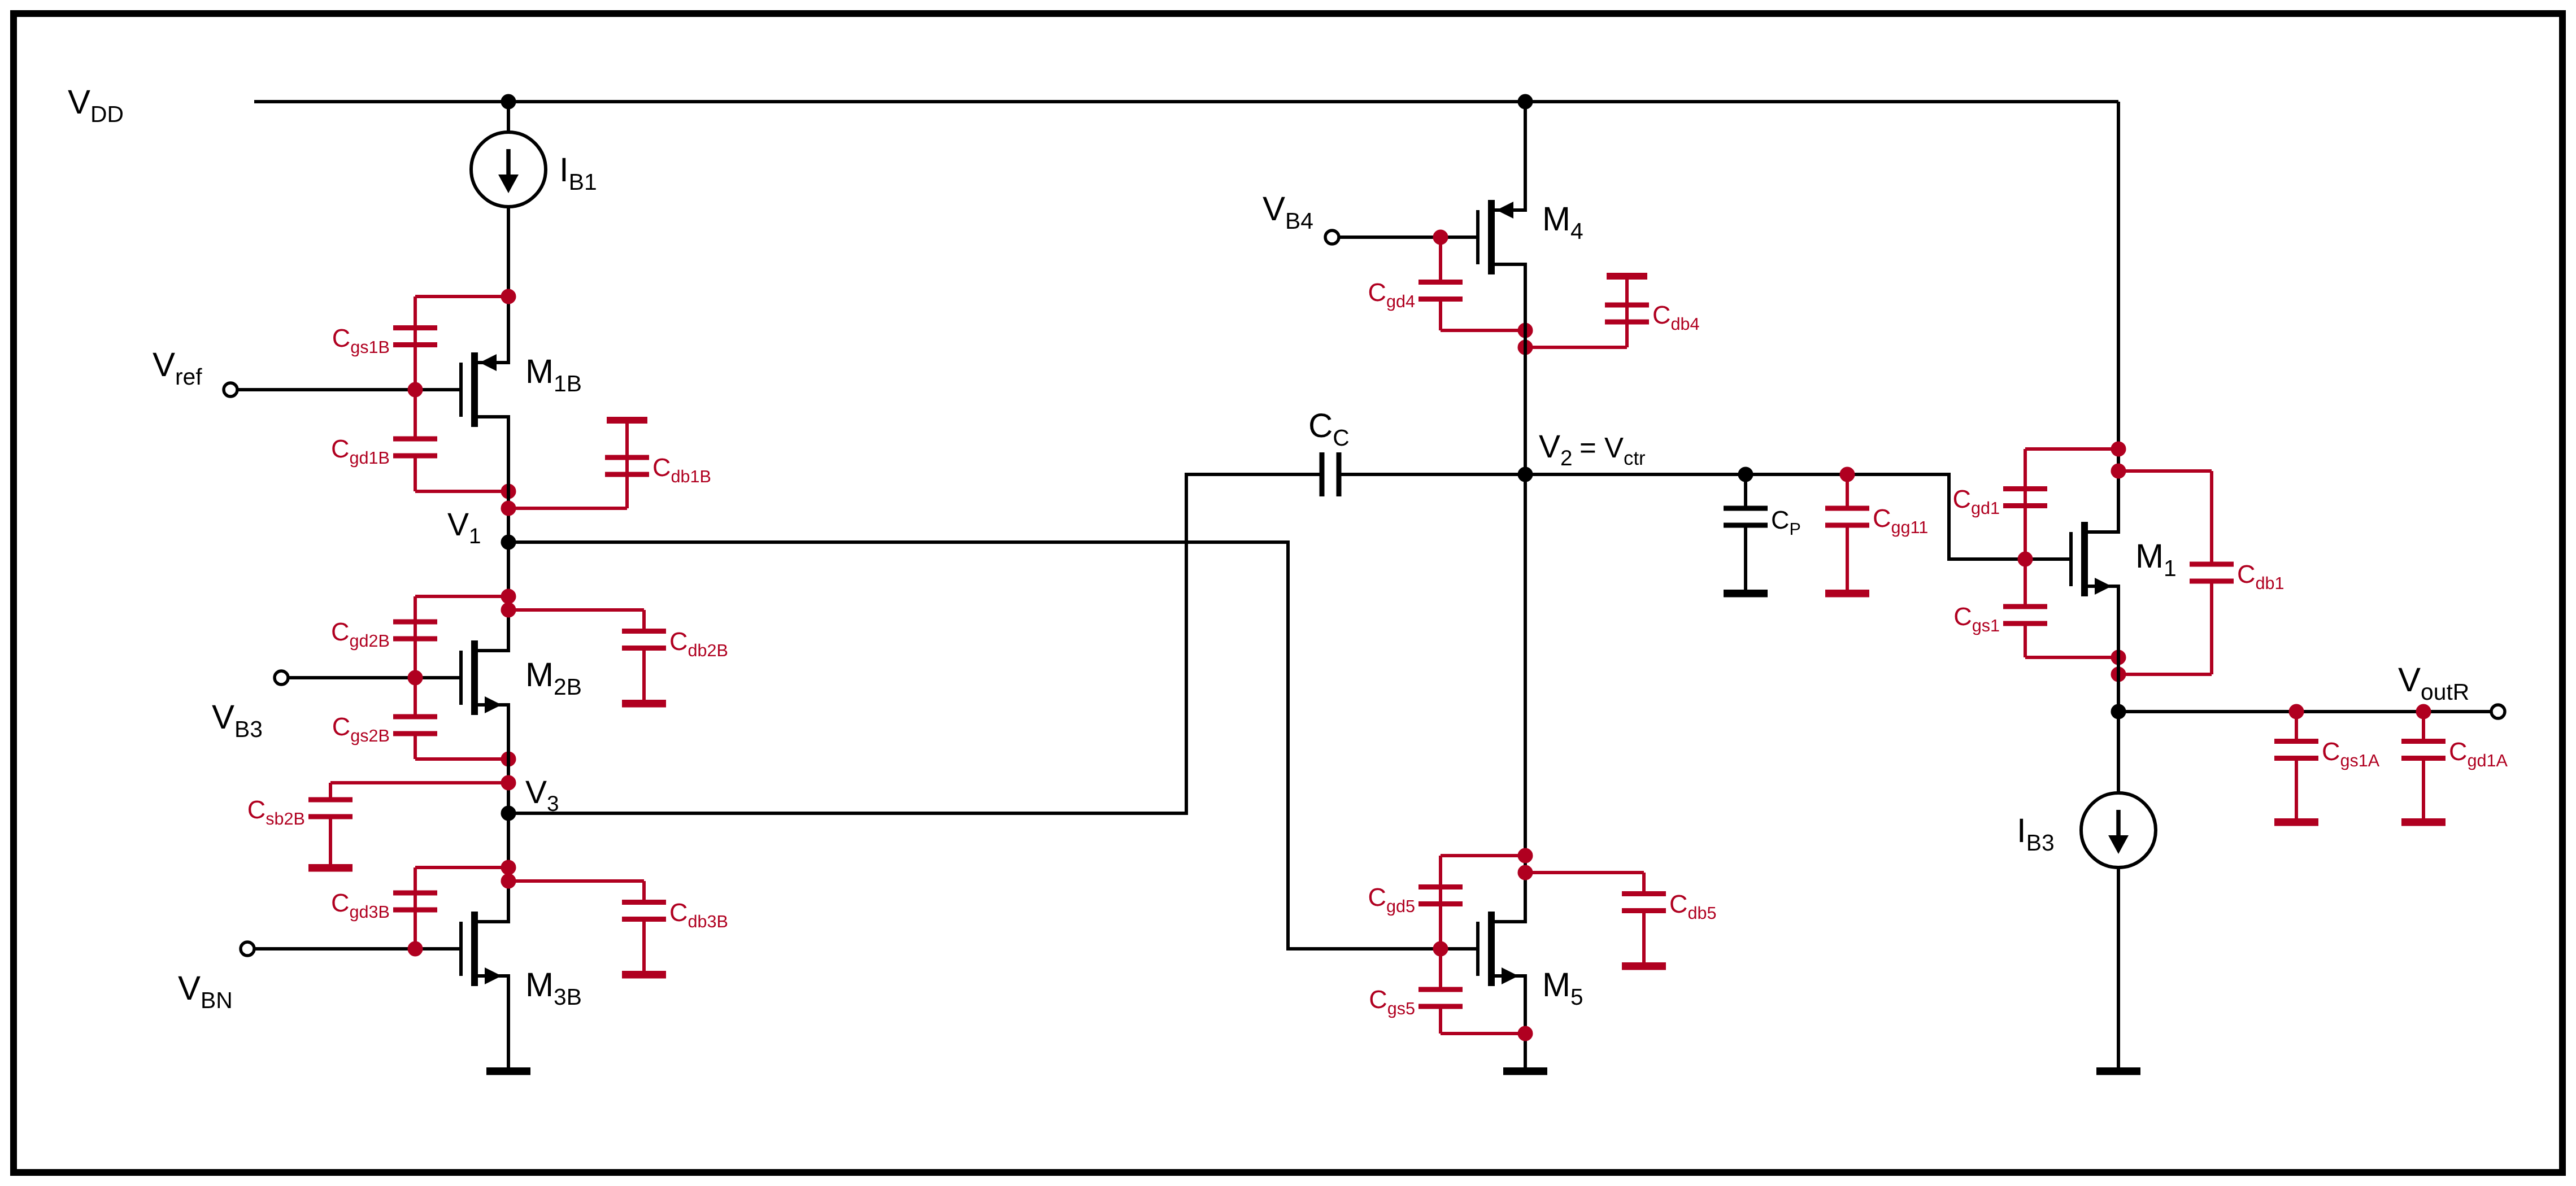
\includegraphics[width=\linewidth]{IMAGENS/circuito_simplificado_parasitas.png}
    \caption{Circuito simplificado do amplificador com as capacidades parasitas.}
    \label{fig:amplificador_parasitas}
\end{figure}

Com o circuito simplificado definido, substitui-se cada transístor pelo seu modelo de pequeno sinal: uma fonte de corrente
controlada $g_m v_{gs}$ entre dreno e fonte, a condutância de saída $g_{ds}$ e as capacidades parasitas da Fig.~\ref{fig:amplificador_parasitas}.
As fontes de polarização ($V_{B3}$, $V_{BN}$, $V_{B4}$ e $V_{DD}$) são ground AC, e as fontes de corrente ideais são circuitos abertos.
Aplica-se então a lei dos nós em $V_1$, $V_2$, $V_3$ e $V_{outR}$, tendo em conta que
\begin{equation*}
    v_{gs1B} = v_{ref}, \qquad v_{gs2B} = -v_3, \qquad v_{gs3B} = v_{gs4} = 0, \qquad v_{gs5} = v_1, \qquad v_{gs1} = v_2 - v_{outR}
\end{equation*}

\textbf{Nó $V_1$:}
\begin{equation}
\begin{gathered}
    0 = v_{ref}\left(g_{m1B} - sC_{gd1B}\right) + v_2\left(-sC_{gd5}\right) + v_3\left(-g_{m2B} - g_{ds2B} - sC_{db2B}\right) \\
    + \, v_1\left(g_{ds1B} + g_{ds2B} + sC_{db1B} + sC_{db2B} + sC_{gd1B} + sC_{gd2B} + sC_{gd5} + sC_{gs5}\right)
\end{gathered}
\end{equation}

\textbf{Nó $V_2$ ($V_{ctr}$):}
\begin{equation}
\begin{gathered}
    0 = v_1\left(g_{m5} - sC_{gd5}\right) + v_3\left(-sC_C\right) + v_{outR}\left(-sC_{gs1}\right) \\
    + \, v_2\big(g_{ds4} + g_{ds5} + sC_{gd5} + sC_{db5} + sC_{db4} + sC_{gd4} \\
    + \, sC_P + sC_{gs11} + sC_{gd11} + sC_{gs1} + sC_{gd1} + sC_C\big)
\end{gathered}
\end{equation}

\textbf{Nó $V_3$:}
\begin{equation}
\begin{gathered}
    0 = v_1\left(-g_{ds2B} - sC_{db2B}\right) + v_2\left(-sC_C\right) \\
    + \, v_3\left(g_{m2B} + g_{ds2B} + g_{ds3B} + sC_{gs2B} + sC_{gd3B} + sC_{db3B} + sC_{db2B} + sC_C\right)
\end{gathered}
\end{equation}

\textbf{Nó $V_{outR}$:}
\begin{equation}
\begin{gathered}
    0 = v_2\left(-g_{m1} - sC_{gs1}\right) \\
    + \, v_{outR}\left(g_{m1} + g_{ds1} + g_{ds,IB3} + sC_{gs1} + sC_{db1} + sC_{db,IB3} + sC_{gs1A} + sC_{gd1A}\right)
\end{gathered}
\end{equation}

O sistema formado pelas quatro equações anteriores foi resolvido simbolicamente em Python, pela regra de Cramer,
para obter o ganho de malha $T(s) = v_{outR}/v_{ref}$.
O resultado é uma razão de polinómios em $s$, com denominador de 4.ª ordem, cujos coeficientes
dependem de todas as transcondutâncias, condutâncias e capacidades do circuito.
As expressões exatas do ganho, dos polos e dos zeros são, por isso, demasiado extensas para serem
apresentadas e interpretadas, pelo que se recorre a um modelo simplificado.

\subsubsection{Modelo simplificado e expressões aproximadas}
\label{subsubsec:aproximadas}

Para obter expressões que relacionem o ganho, o GBW e os polos com os parâmetros de cada transístor, e que possam ser
usadas no dimensionamento, simplifica-se o modelo com as seguintes hipóteses:
\begin{itemize}
    \item $g_{ds} \ll g_m$ em todos os transístores;
    \item as capacidades parasitas flutuantes ($C_{gd1B}$, $C_{db2B}$, $C_{gd5}$) são desprezáveis face a $C_C$;
    \item o seguidor réplica tem ganho aproximadamente unitário e um polo muito acima do GBW, pelo que $v_{outR} \approx v_{ctr}$.
    Por isso, a tensão aos terminais de $C_{gs1}$ quase não varia e esta capacidade pode ser desprezada.
\end{itemize}

\begin{figure}[H]
    \centering
    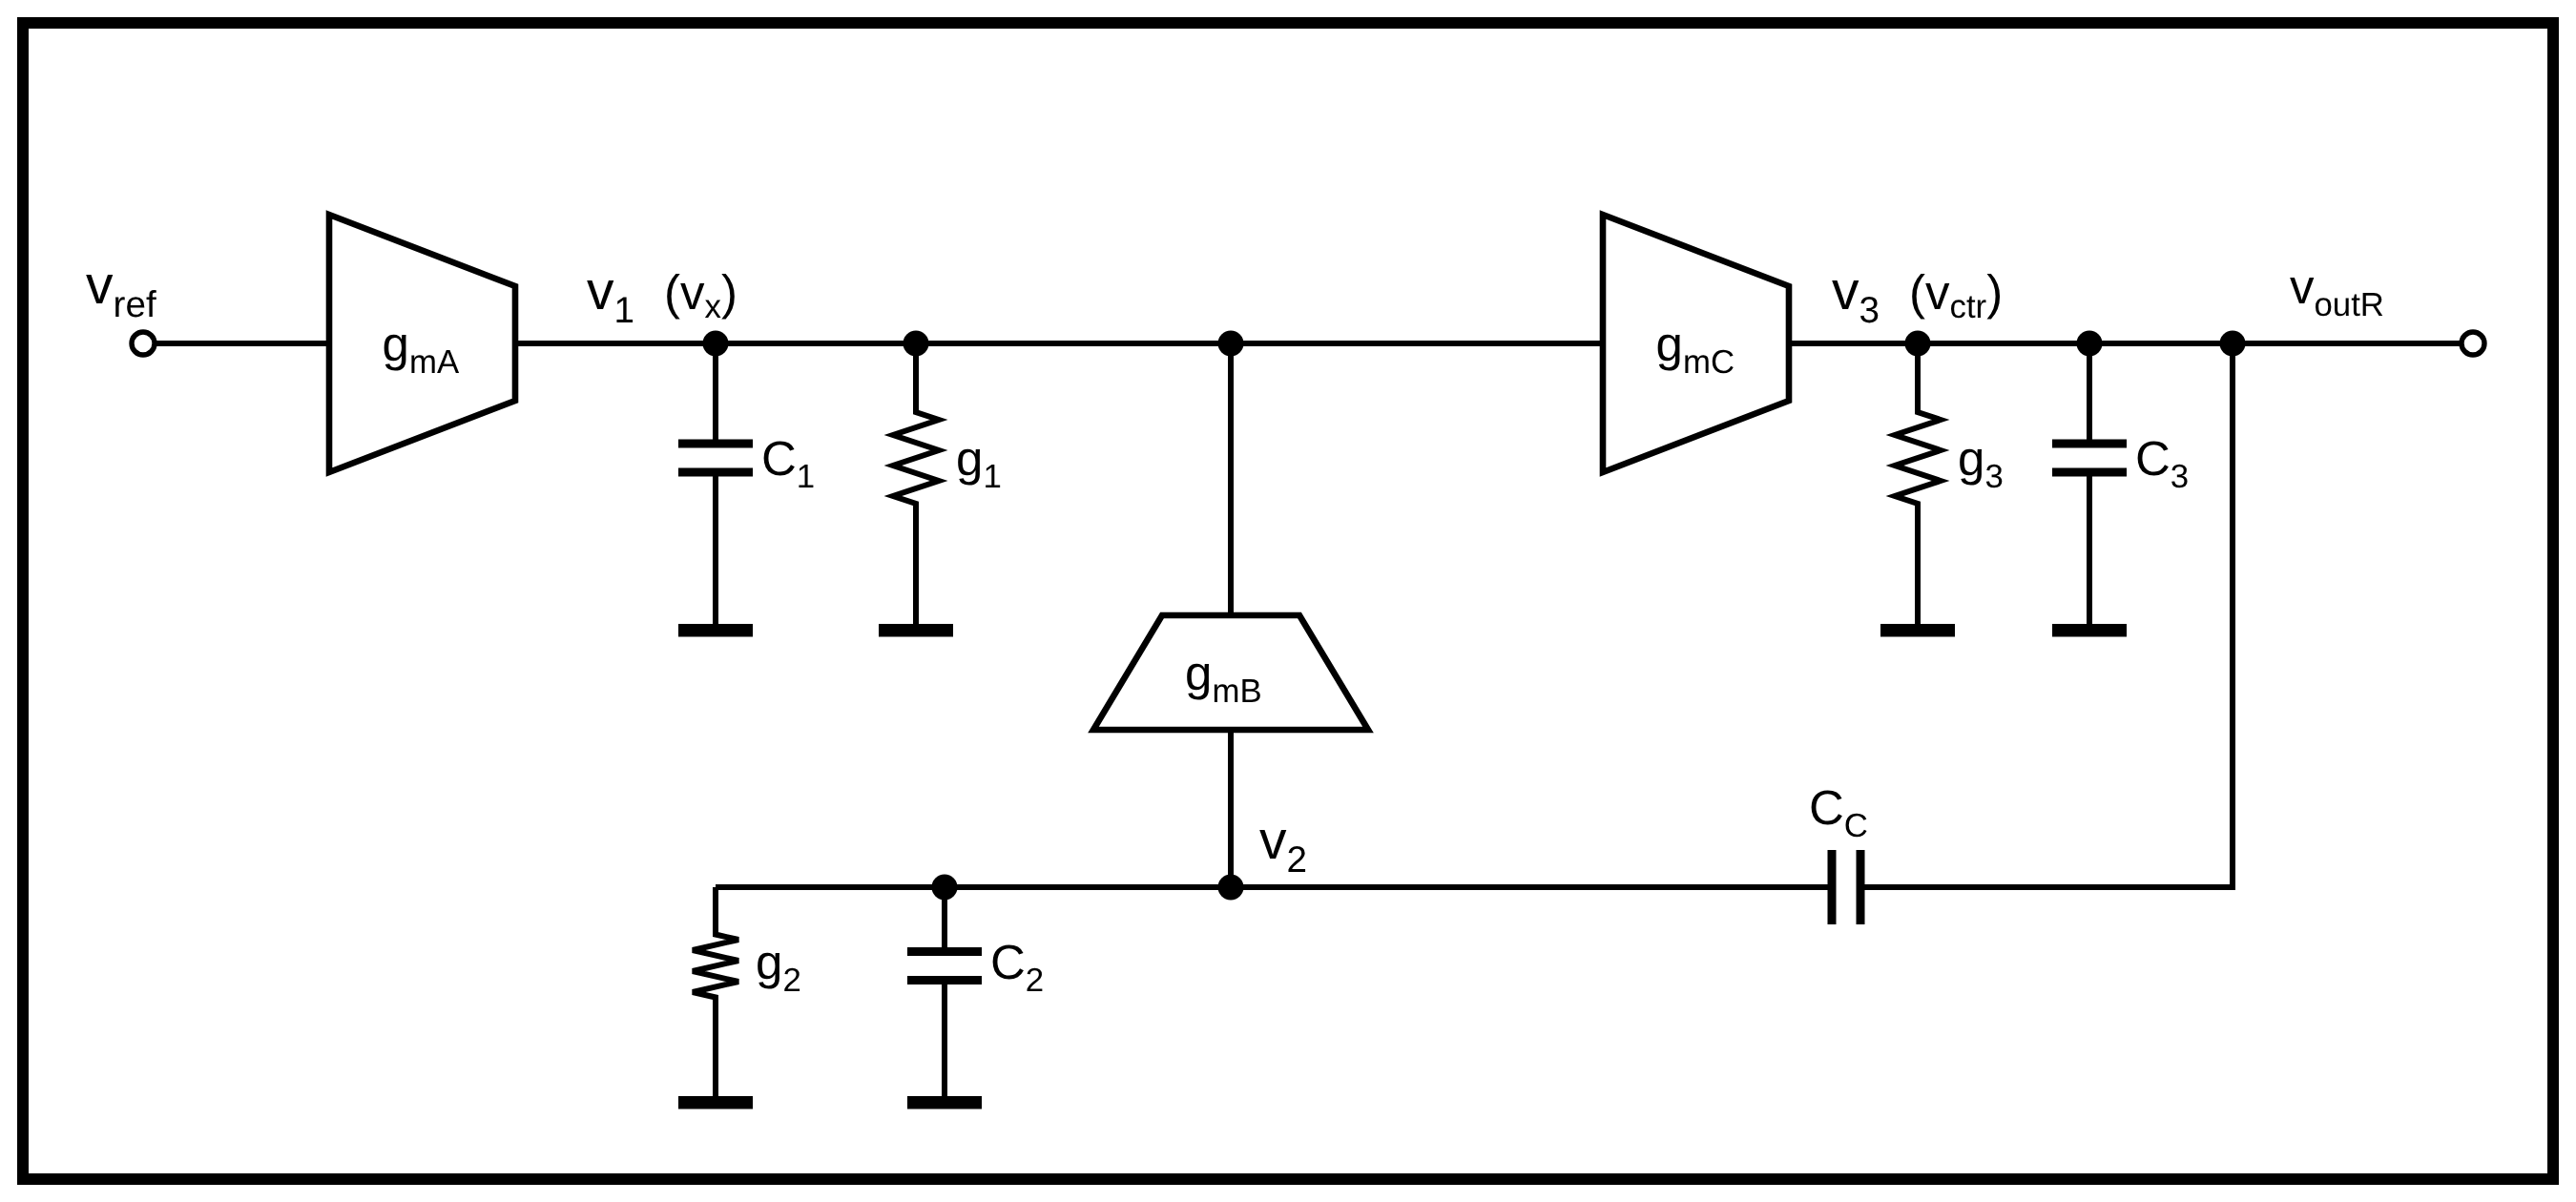
\includegraphics[width=0.85\linewidth]{IMAGENS/modelo_simplificado.png}
    \caption{Modelo simplificado do amplificador.}
    \label{fig:modelo_simplificado}
\end{figure}

Com estas hipóteses, cada transístor é reduzido a uma transcondutância e a uma condutância e capacidade equivalentes em cada nó, obtendo-se o modelo da
Fig.~\ref{fig:modelo_simplificado}. Neste modelo, o nó $v_1$ corresponde a $V_x$, o nó $v_2$ à fonte da cascode $M_{2B}$ e o nó $v_3$ a $V_{ctr}$.


\paragraph{Transcondutâncias.}
O par de entrada $M_{1B}$ converte $v_{ref}$ numa corrente injetada em $v_1$, e o andar de fonte comum $M_5$ converte $v_1$ numa corrente injetada em $v_3$:
\begin{equation}
    g_{mA} = g_{m1B}, \qquad g_{mC} = g_{m5}
\end{equation}
A compensação é feita através da cascode: $C_C$ liga $V_{ctr}$ à fonte de $M_{2B}$, um nó de baixa impedância. Assim, $M_{2B}$ funciona como \textit{buffer} de corrente: a corrente que atravessa $C_C$ entra pela fonte de $M_{2B}$ e é transferida para o nó $v_1$ com transcondutância
\begin{equation}
    g_{mB} = g_{m2B} + g_{mb2B}
\end{equation}
onde se inclui o efeito de corpo de $M_{2B}$, cujo \textit{bulk} está ligado a terra.

\paragraph{Condutâncias.}
No nó $v_1$ ligam-se a condutância de saída de $M_{1B}$ e a resistência vista para dentro da cascode, $g_{casc} = g_{ds2B}\,g_{ds3B}/g_{m2B}$. Como $g_m \gg g_{ds}$, $g_{casc}$ é desprezável:
\begin{equation}
    g_1 = g_{ds1B} + \frac{g_{ds2B}\,g_{ds3B}}{g_{m2B}} \approx g_{ds1B}
\end{equation}
No nó $v_2$ (fonte de $M_{2B}$), a condutância é dominada pela própria transcondutância da cascode:
\begin{equation}
    g_2 = g_{m2B} + g_{mb2B} + g_{ds2B} + g_{ds3B} \approx g_{mB}
\end{equation}
No nó $v_3$ ($V_{ctr}$), $M_4$ é uma fonte de corrente com a gate fixa ($v_{gs4} = 0$), pelo que contribui apenas com a sua condutância de saída:
\begin{equation}
    g_3 = g_{ds4} + g_{ds5}
\end{equation}

\paragraph{Capacidades.}
Agrupando as capacidades parasitas de cada nó para terra:
\begin{align}
    C_1 &= C_{db1B} + C_{gd2B} + C_{gs5} \\
    C_2 &= C_{gs2B} + C_{sb2B} + C_{gd3B} + C_{db3B} \\
    C_3 &= C_{db4} + C_{gd4} + C_{db5} + C_P + C_{gs11} + C_{gd11} + C_{gd1}
\end{align}
Note-se que $C_3$ inclui a carga do seguidor de saída ($C_{gg11} = C_{gs11} + C_{gd11}$), que é a contribuição dominante deste nó.

\paragraph{Equações dos nós.}
Aplicando a lei dos nós ao modelo da Fig.~\ref{fig:modelo_simplificado}:
\begin{align}
    v_1:&\quad g_{mA}\,v_{ref} + v_1\left(g_1 + sC_1\right) - g_{mB}\,v_2 = 0 \\
    v_2:&\quad v_2\left(g_2 + sC_2\right) + sC_C\left(v_2 - v_3\right) = 0 \\
    v_3:&\quad g_{mC}\,v_1 + v_3\left(g_3 + sC_3\right) + sC_C\left(v_3 - v_2\right) = 0
\end{align}
Resolvendo o sistema (Python, regra de Cramer) obtém-se uma função de transferência com um zero e três polos. Considerando que os
polos estão bem separados, cada polo é aproximado pela razão entre coeficientes consecutivos do denominador,
$p_k \approx -a_{k-1}/a_k$, resultando em:
\begin{align}
    A_0 &= \frac{g_{mA}\,g_{mC}}{g_1\,g_3} = \frac{g_{m1B}}{g_{ds1B}}\cdot\frac{g_{m5}}{g_{ds4}+g_{ds5}} \label{eq:A0_aprox}\\
    GBW &= \frac{g_{mA}}{2\pi\,C_C} = \frac{g_{m1B}}{2\pi\,C_C} \label{eq:gbw}\\
    p_1 &\approx -\frac{g_1\,g_3}{g_{mC}\,C_C} \\
    p_2 &\approx -\frac{g_{mC}\,C_C}{C_1\left(C_3 + C_C\right)} \label{eq:p2}\\
    p_3 &\approx -\frac{g_{mB}\left(C_3 + C_C\right)}{C_3\,C_C} \label{eq:p3}\\
    z_1 &= -\frac{g_{mB}}{C_C + C_2}
\end{align}

O zero $z_1$ está no semiplano esquerdo: ao contrário da compensação de Miller clássica, em que $C_C$ liga diretamente a
saída do primeiro andar e cria um zero no semiplano direito, aqui a corrente de $C_C$ passa pela cascode, o que elimina esse
zero e contribui com avanço de fase. O polo $p_2$ é o principal não dominante e depende sobretudo de $g_{m5}$, enquanto $p_3$ é introduzido pela cascode e depende de $g_{mB}$.
Estas expressões são usadas no dimensionamento da secção seguinte.

% ========== DIMENSIONAMENTO DO RESTO ==========
% ========== Alínea e) ==========
\subsection{Dimensionamento pela metodologia \texorpdfstring{$g_m/I_D$}{gm/ID}}
\label{subsec:gmid}

\subsubsection{Especificações e critérios}
\label{subsubsec:criterios}

O amplificador tem de cumprir $GBW > 100$~MHz, $A_0 > 46$~dB e uma margem de fase de $60^\circ$,
com a menor corrente possível. Para transformar estas especificações em condições sobre cada
transístor, usam-se as expressões aproximadas da Secção~\ref{subsubsec:aproximadas}.

\paragraph{Capacidade de compensação.} Define-se $C_C$ em função da capacidade do nó de saída
através de um fator $\alpha$:
\begin{equation}
    C_C = \alpha\,C_3
\end{equation}

Escolheu-se inicialmente $\alpha = 1$, pois além da facilidade em cálculos, equilibra o esforço entre os dois andares: valores
maiores de $\alpha$ aumentam $C_C$ e, com ele, o $g_{m1B}$ necessário, enquanto valores menores
exigem um $M_5$ mais rápido. A capacidade $C_3$ é dominada pela carga dos seguidores ($C_{gg11}
\approx C_{gg1} \approx 2{,}42$~pF) e pelo condensador $C_P$, que se fixou inicialmente em
$C_P = 10\,C_{gg11}$, de modo a que $V_{ctr}$ seja pouco perturbado pela ligação de $C_{DAC}$.

\paragraph{GBW.} Da Eq.~\eqref{eq:gbw}, o GBW fixa a transcondutância do par de entrada:
\begin{equation}
    g_{m1B} \ge 2\pi \cdot GBW \cdot C_C
    \label{eq:cond_gm1b}
\end{equation}

\paragraph{Margem de fase.} Para uma margem de fase de $60^\circ$, o polo não dominante $p_2$ tem
de estar a pelo menos $2{,}5$ vezes o GBW. Da Eq.~\eqref{eq:p2}, e separando $C_1 = C_x + C_{gs5}$,
onde $C_x$ representa as capacidades de $M_{1B}$ e $M_{2B}$ no nó $V_x$ e $C_{gs5} \approx g_{m5}/(2\pi f_{T5})$:
\begin{equation}
    \frac{g_{m5}\,C_C}{\left(C_x + C_{gs5}\right)\left(C_3 + C_C\right)} \ge 2{,}5 \cdot 2\pi\,GBW
\end{equation}

Resolvendo em ordem a $g_{m5}$:
\begin{equation}
    g_{m5} \ge \frac{2{,}5 \cdot 2\pi\,GBW \left(1 + \frac{1}{\alpha}\right) C_x}{1 - \dfrac{f_{T5,min}}{f_{T5}}},
    \qquad f_{T5,min} = 2{,}5\,GBW\left(1 + \frac{1}{\alpha}\right)
    \label{eq:cond_gm5}
\end{equation}

A frequência de transição de $M_5$ tem, por isso, de ser bem superior a $f_{T5,min}$ (500~MHz para $\alpha = 1$),
caso contrário o $g_{m5}$ necessário cresce sem limite.

Adicionalmente, o polo da cascode $p_3$ deve ficar acima de $4\,GBW$. Da Eq.~\eqref{eq:p3}:
\begin{equation}
    g_{m2B} + g_{mb2B} \ge 2\pi \cdot 4\,GBW \cdot \frac{C_3\,C_C}{C_3 + C_C}
    \label{eq:cond_gm2b}
\end{equation}

\paragraph{Ganho DC.} Da Eq.~\eqref{eq:A0_aprox}, o ganho é o produto dos ganhos dos dois andares:
\begin{equation}
    A_0 = A_1 \cdot A_2 = \frac{g_{m1B}}{g_{ds1B}}\cdot\frac{g_{m5}}{g_{ds4} + g_{ds5}} \ge 200 \quad (46~\text{dB})
\end{equation}
Uma divisão igual corresponderia a $A_1 = A_2 = \sqrt{A_0} \approx 14$. No entanto, os dois andares não são equivalentes.
No primeiro, a cascode torna desprezável a condutância da carga, pelo que $A_1 \approx (g_m/g_{ds})_{1B}$. No segundo,
a carga $M_4$ contribui com uma condutância da mesma ordem da de $M_5$, e $M_5$ precisa de um $f_T$ elevado (Eq.~\eqref{eq:cond_gm5}),
o que limita o seu $g_m/g_{ds}$. Optou-se, por isso, por atribuir a maior parte do ganho ao primeiro andar:
\begin{equation}
    A_1 = 2\sqrt{A_0} \approx 28, \qquad A_2 = \frac{\sqrt{A_0}}{2} \approx 7
\end{equation}
Considerando $g_{ds4} \approx g_{ds5}$, isto impõe
\begin{equation}
    \left(\frac{g_m}{g_{ds}}\right)_{1B} \ge 28, \qquad
    \left(\frac{g_m}{g_{ds}}\right)_{5} \ge 2A_2 \approx 14
\end{equation}

\paragraph{Margens de tensão.} Todos os transístores têm de operar em saturação. Os nós críticos são $V_{ctr} \approx 1{,}554$~V,
que deixa a $M_4$ apenas $V_{SD4} = V_{DD} - V_{ctr} \approx 0{,}25$~V, e $V_x = V_{GS5}$, que tem de acomodar $V_{DSAT2B} + V_{DSAT3B}$.
Pela mesma razão, a fonte do par diferencial está a $V_{ref} + V_{SG1B}$, o que limita $V_{SG1B}$ para que a fonte de cauda permaneça saturada.

\paragraph{Metodologia.} Para cada transístor, as condições anteriores que não dependem do tamanho
($g_m/I_D$, $f_T$, $g_m/g_{ds}$, $V_{DSAT}$, $V_{GS}$) servem para escolher o ponto de funcionamento numa tabela
obtida por simulação de um transístor de referência ($W = 2~\mu$m $\times$ 5 \textit{fingers}).
O tamanho final é obtido através do multiplicador $M$, escolhido de forma a atingir o $g_m$ ou a corrente necessários:
\begin{equation}
    M = \frac{g_m}{g_{m,tab}} = \frac{I_D}{I_{D,tab}}
\end{equation}

Como os transístores em paralelo mantêm a mesma densidade de corrente, $g_m/I_D$, $f_T$, $g_m/g_{ds}$ e $V_{DSAT}$ não se alteram com $M$.


% ========== ESCOLHA DE CADA TRANSISTOR DO AMPLIFICADOR ==========
\subsubsection{Escolha de cada transístor}
\label{subsubsec:escolha}

Com $C_P = 10\,C_{gg11}$ e $C_{gg1} = C_{gg11} = 2{,}417$~pF, a capacidade do nó de saída é $C_3
\approx C_P + C_{gg11} + C_{gg1} = 12\,C_{gg11} \approx 29{,}0$~pF e, com $\alpha = 1$,
$C_C = 29{,}0$~pF.

\paragraph{$M_5$ (segundo andar).}
$M_5$ converte a tensão em $V_x$ numa corrente que carrega o nó $V_{ctr}$: define o ganho do
segundo andar e o polo não dominante $p_2$. Das condições da Secção~\ref{subsubsec:criterios},
o seu ponto de funcionamento tem de cumprir:
\begin{itemize}
    \item $f_{T5} = \dfrac{g_{m5}}{2\pi\,C_{gg5}} > f_{T5,min} = 500$~MHz (para $\alpha = 1$),
    para que $p_2$ possa ser colocado a $2{,}5\,GBW$;
    \item $(g_m/g_{ds})_5 \ge 14$, para o ganho do segundo andar;
    \item $V_{GS5} \ge 0{,}55$~V. Como $V_x = V_{GS5}$ e este nó alimenta a cascode, tem de se verificar $V_{GS5} > V_{DSAT2B} + V_{DSAT3B} \approx 0{,}4$~V; usou-se 0,55~V para garantir margem adicional.
\end{itemize}

Entre os pontos que cumprem estas condições, escolheu-se o que exige a menor corrente total.
Para cada ponto, calcula-se o $g_{m5}$ necessário pela Eq.~\eqref{eq:cond_gm5} e a corrente
$I_{D5} = g_{m5}/(g_m/I_D)$. Note-se que o ponto de menor corrente não é o de maior $g_m/I_D$:
um $g_m/I_D$ elevado reduz $f_{T5}$ e, pelo denominador da Eq.~\eqref{eq:cond_gm5}, aumenta o
$g_{m5}$ necessário. Escolheu-se o ponto com $L = 0{,}5~\mu$m, $g_m/I_D = 10{,}9$~V$^{-1}$, $V_{GS}
= 0{,}59$~V, $f_T = 2{,}48$~GHz e $g_m/g_{ds} = 20$. Com a capacidade do nó $V_x$ (sem $C_{gs5}$)
estimada em $C_x \approx 1{,}49$~pF a partir de $M_{1B}$, $M_{2B}$ e das fontes $I_{extra}$,
obtém-se $g_{m5} \ge 5{,}87$~mS, $M = 8$ e $I_{D5} = 548~\mu$A.

\paragraph{$M_4$, $M_{4A}$ e $M_{4B}$ (espelho PMOS).}
$M_4$ é a carga ativa do segundo andar. Como tem a gate a uma tensão fixa, não contribui com sinal:
entra apenas através de $g_{ds4}$, no ganho, e da sua capacidade de dreno, no nó $V_{ctr}$. Por isso
usa-se um $g_m/I_D$ moderado, limitado pela margem de tensão, $V_{SD4} = V_{DD} - V_{ctr} \approx
0{,}25$~V, o que impõe $V_{DSAT4} \le 0{,}18$~V ($g_m/I_D \approx 10$--15~V$^{-1}$). Entre os pontos
possíveis escolheu-se o de maior $g_m/g_{ds}$, para maximizar o ganho, e menor tamanho: $L = 2~\mu$m,
$g_m/I_D = 14{,}9$~V$^{-1}$, $g_m/g_{ds} = 21{,}3$ e $V_{DSAT} = 94$~mV. Como $I_{D4} = I_{D5}$,
resulta $M = 95$.

$M_{4A}$ é o díodo de referência do espelho, com $M = 10$ e $I_B = 57{,}5~\mu$A, e a fonte de cauda
$M_{4B}$ usa o mesmo ponto e o mesmo $L$. O seu multiplicador é definido pela corrente de cauda,
$I_{B1} = 2\,I_{D1B}$ (ver abaixo), resultando $M = 294$.

\paragraph{$M_{1A}$ e $M_{1B}$ (par de entrada).}
O par diferencial converte a diferença entre $V_{ref}$ e $V_{outR}$ numa corrente injetada em $V_x$,
definindo o GBW e o ganho do primeiro andar. Pela Eq.~\eqref{eq:cond_gm1b}, $g_{m1B} \ge 2\pi
\cdot 100~\text{MHz} \cdot 29{,}0~\text{pF} \approx 18{,}2$~mS. O ponto de funcionamento tem de
cumprir:
\begin{itemize}
    \item $(g_m/g_{ds})_{1B} \ge 28$, para o ganho do primeiro andar;
    \item $|V_{GS1B}| \le 0{,}55$~V, para que a fonte de cauda, com $V_{SD} = V_{DD} - V_{ref} - V_{SG1B}$, permaneça saturada.
\end{itemize}

Como $g_{m1B}$ está fixo, a menor corrente corresponde ao maior $g_m/I_D$, já que $I_{D1B} =
g_{m1B}/(g_m/I_D)$. Escolheu-se o ponto com $L = 0{,}5~\mu$m, $g_m/I_D = 21{,}6$~V$^{-1}$,
$g_m/g_{ds} = 33{,}5$ e $V_{SG} = 0{,}44$~V. Comprimentos maiores davam um $g_m/I_D$ praticamente
igual, mas com transístores muito maiores e mais capacidade em $V_x$. Resulta $M = 266$, com
$I_{D1B} = 844~\mu$A e $I_{B1} \approx 1{,}69$~mA.

\paragraph{$M_{2A}$ e $M_{2B}$ (cascode) e fonte $I_{extra}$.}
A cascode isola $V_x$ da fonte de corrente $M_{3B}$ e é o caminho da corrente de compensação,
definindo $p_3$ e $z_1$. Pela Eq.~\eqref{eq:cond_gm2b}, com $\alpha = 1$, $g_{m2B} + g_{mb2B}
\ge 2\pi \cdot 200~\text{MHz} \cdot C_C \approx 36{,}4$~mS, ou seja, cerca do dobro de $g_{m1B}$.
Se $M_{2B}$ conduzisse a mesma corrente que $M_{1B}$, seria necessário um $g_m/I_D$ próximo de
43~V$^{-1}$, acima do máximo teórico. Por isso, adiciona-se uma fonte de corrente $I_{extra}$ a
injetar no nó $V_x$ (Fig.~\ref{fig:amplificador_iextra}), de modo que
\begin{equation}
    I_{D2B} = I_{D3B} = I_{D1B} + I_{extra}
\end{equation}
Em pequeno sinal, esta fonte apenas acrescenta a sua condutância e capacidade de saída ao nó $V_x$,
pelo que as expressões da Secção~\ref{subsubsec:aproximadas} se mantêm.

\begin{figure}[H]
    \centering
    \includegraphics[width=0.8\linewidth]{IMAGENS/circuito_simplificado_com_Iextra.png}
    \caption{Circuito simplificado do amplificador com a fonte $I_{extra}$.}
    \label{fig:amplificador_iextra}
\end{figure}

O ponto de $M_{2B}$ tem de cumprir $V_{DSAT} \le 0{,}18$~V (tem de caber em $V_x$ juntamente com
$M_{3B}$), $(g_m/g_{ds})_{2B} \ge 10$ (suficiente para a cascode tornar $g_{ds3B}$ desprezável) e
$f_{T2B} \ge 2$~GHz, bem acima de $p_3$, para que as capacidades do próprio transístor não reduzam
este polo. Entre estes, escolheu-se o que exige a menor corrente: $L = 0{,}3~\mu$m,
$g_m/I_D = 17{,}8$~V$^{-1}$, $V_{DSAT} = 79$~mV e $f_T = 2{,}15$~GHz, que resulta em $M = 98$ e
$I_{D2B} \approx 1{,}76$~mA.

\paragraph{$M_{3A}$ e $M_{3B}$ (fonte de corrente).}
$M_{3B}$ é a fonte de corrente na base do ramo: fixa a corrente $I_{D2B}$, mas não contribui para o
ganho nem para os polos do modelo simplificado. Escolheu-se, por isso, um $g_m/I_D$ baixo
($\approx 10$--13~V$^{-1}$), que reduz o ruído e o tamanho, com $V_{DSAT} \le 0{,}2$~V, e um
comprimento maior, para melhorar o emparelhamento entre $M_{3A}$ e $M_{3B}$. Entre os pontos possíveis
escolheu-se o de menor capacidade de dreno: $L = 1~\mu$m, $g_m/I_D = 10{,}0$~V$^{-1}$ e $V_{DSAT} =
151$~mV, com $M = 41$ ($I_{D3B} = 1{,}76$~mA). Resulta $I_{extra} = I_{D3B} - I_{D1B} \approx
915~\mu$A em cada ramo.

Na simulação, as fontes $I_{extra}$ foram implementadas como fontes de corrente ideais; num circuito
real seriam saídas adicionais do espelho de $M_{4A}$.


% ========== Alíneas g) e h) ==========
\subsection{Simulação do amplificador}
\label{subsec:sim_amp}

\subsubsection{Ponto de funcionamento}
\subsubsection{Resposta em frequência em malha aberta}
\subsubsection{Otimização do consumo}

% ========== Alíneas f) e i) ==========
\subsection{Impedância de saída}
\label{subsec:zout}

\subsubsection{Análise teórica}
\subsubsection{Simulação}

% ========== Alíneas j) e k) ==========
\subsection{Ruído e PSRR}
\label{subsec:ruido_psrr}

\subsubsection{Ruído de saída}
\subsubsection{PSRR$^+$}

% ========== Alínea l) ==========
\subsection{Funcionamento no tempo}
\label{subsec:tran}

% ========== Resumo ==========
\subsection{Resumo do desempenho}
\label{subsec:resumo}